\section{مسئله سه‌جسمی محدود دایره‌ای}

%مسئله عمومی سه‌جسمی مسیرهای سه جسم پرجرم دلخواه را بررسی می‌کند که تحت تأثیر جاذبه متقابل قرار دارند. با این حال، این مسئله به مراتب عمومی‌تر از آن چیزی است که طراحان مأموریت‌های عملیاتی نیاز دارند. دو ساده‌سازی رایج وجود دارد که برای قابل دسترس‌تر و کاربردی‌تر کردن این مسئله در مسیرهای واقعی معمولاً انجام می‌شود. این ساده‌سازی‌ها عبارتند از:
%\begin{enumerate}
%	\item جرم جسم سوم (ماهواره) در مقایسه با اجسام اصلی ناچیز است.
%	\item اجسام اصلی و ثانویه در مدارهای دایره‌ای حول مرکز جرم که بین دو جسم قرار دارد حرکت می‌کنند.
%\end{enumerate}
%
%مسئله به‌دست‌آمده معمولاً به نام مسئله سه‌جسمی محدود دایره‌ای (CRTBP) شناخته می‌شود. گاهی اوقات، فرض دیگری نیاز به حرکت فقط در صفحه مداری اجسام اصلی و ثانویه دارد. برای این مسئله سه‌جسمی محدود دایره‌ای در صفحه، مؤلفه z معادلات صفر می‌شود. پیدا کردن معادلات ساده برای بیان راه‌حل‌ها در مسئله سه‌جسمی دشوار است. کتاب‌های کامل در این زمینه وجود دارد (Szebehely, 1967). هدف ما در اینجا توصیف حرکات کیفی و برجسته کردن چندین راه‌حل کلاسیکی است که شناخته‌شده هستند.
%
%ابتدا، بیایید از یک چارچوب مختصات همزمان برای مسئله سه‌جسمی استفاده کنیم، همانطور که در شکل 12-13 نشان داده شده است.* معادلاتی برای یک چارچوب باریکنانه (ثابت) به زودی معرفی خواهیم کرد. این چارچوب از نمادهای کوچک x، y و z برای اجزای فردی استفاده می‌کند. زیرنویس S با محور‌ها نشان می‌دهد که مبدأ در مرکز جرم (مرکز سیستم) است و چارچوب با سرعت زاویه‌ای qS می‌چرخد.

%Macros
\pgfmathsetmacro{\r}{0.8}	
\pgfmathsetmacro{\Phi}{-160}
\pgfmathsetmacro{\Theta}{-90}

\begin{figure}[H]
	\centering
	\begin{tikzpicture}
		%Grid
		%		\draw[thin, dotted] (0,0) grid (8,8);
		%		\foreach \i in {1,...,8}
		%		{
			%			\node at (\i,-2ex) {\i};	
			%		}
		%		\foreach \i in {1,...,8}
		%		{
			%			\node at (-2ex,\i) {\i};	
			%		}
		%		\node at (-2ex,-2ex) {0};
		
		% Coordinates
		\coordinate (earth) at (1,2);
		\coordinate (moon) at (8,1);
		\coordinate (earth-point1) at ({\r*cos(\Theta)+1},{\r*sin(\Theta)+2});
		\coordinate (A) at (-.5,.5);
		\coordinate (B) at (8.5,-0.5);
		
		% Earth
		\draw[thick, fill=black!30, draw=black!30
		] (earth) circle (\r);
		\node[inner sep=0pt] (Earth_c) at (earth) {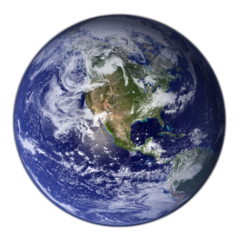
\includegraphics[width=1.8cm]{../Figure/TBP/Earth.png}};
		% Text
		\node[below, shift={(0,-0.8)}] at (earth) {$m_1$};
		\node (a) at (A) {Earth};
		
		% Moon
		\node[circle, inner sep=5.5pt, fill=black!30] (MOON) at (moon) {};
		\node[inner sep=0pt] (moon_c) at (moon) {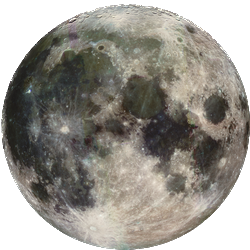
\includegraphics[width=.5cm]{../Figure/TBP/Moon.png}};
		% Text 
		\node[below, shift={(0,-0.4)}] at (MOON) {$m_2$};
		\node (b) at (B) {Moon};
		
		% Lines
		% \draw[-latex] (earth) -- (MOON) node[pos=.55, below left] {$\vb{r}_o$};
		% \draw[-latex] (earth) -- (earth-point1) node [pos=0.6, left] {$\vb{r}$};
		\draw[-stealth] (a) to[bend left=30] ({\r*cos(\Phi)+1},{\r*sin(\Phi)+2});
		\draw[-stealth] (b) to[bend left=-30] (MOON);
		\draw[dashed, black] (earth) -- (MOON.center);
		
		% center of mass 0.25 from earth
		\coordinate (center) at ($(earth)!0.3!(MOON)$);
		% small circle
		\draw[fill=black] (center) circle (1.5pt) node[below, shift={(0,-0.1)}] {Center of Mass};
		% add satellite with shift
		\coordinate (satellite) at ($(center)!0.5!(MOON)+(0,2)$);
		% \node at ($(center)!0.5!(MOON)+(0,2)$) {\faSatellite};
		% shift coordinate
		\node (satellite) at (satellite) {\faSatellite};
		
		% connect earth to satellite r1
		\draw[-stealth] (earth) -- (satellite) node[pos=0.5, above] {$\vb{r}_1$};   
		% connect moon to satellite r2
		\draw[-stealth] (MOON) -- (satellite) node[pos=0.5, above] {$\vb{r}_2$};
		% connect center of mass to satellite r
		\draw[-stealth] (center) -- (satellite) node[pos=0.5, above] {$\vb{r}$};
		% add line to show satellite is in between
		\node (c) at ($(satellite)+(1.5,0.5)$) {Satellite};
		\draw[-stealth] (c) to[bend left=30] (satellite);
		
		
		
		
		
		% % Angles
		% \pic[draw, "$\theta$", angle eccentricity=2.5, angle radius=5pt] {angle = moon--earth--earth-point1};
		
		% % Point
		% \draw[fill=black] (earth) circle (1pt) node[below, shift={(0,-0.1)}] {$\mathrm{O}$};
	\end{tikzpicture}
	\caption{هندسه مسئله سه بدنه محدود}
\end{figure}











\begin{figure}[H]
	\centering
	\begin{tikzpicture}
		% Coordinates
		\coordinate (earth) at (1,2);
		\coordinate (moon) at (8,1);
		\coordinate (earth-point1) at ({\r*cos(\Theta)+1},{\r*sin(\Theta)+2});
		\coordinate (A) at (-.5,.5);
		\coordinate (B) at (8.5,-0.5);
		
		% Earth
		\draw[thick, fill=black!30, draw=black!30
		] (earth) circle (\r);
		\node[inner sep=0pt] (Earth_c) at (earth) {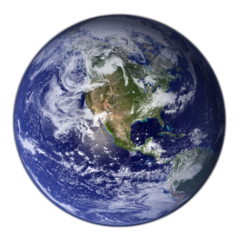
\includegraphics[width=1.8cm]{../Figure/TBP/Earth.png}};
		% Text
		\node[below, shift={(0,-0.8)}] at (earth) {$m_1$};
		\node (a) at (A) {Earth};
		
		% Moon
		\node[circle, inner sep=5.5pt, fill=black!30] (MOON) at (moon) {};
		\node[inner sep=0pt] (moon_c) at (moon) {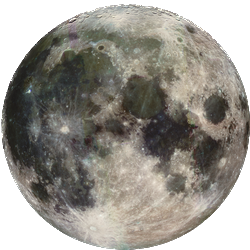
\includegraphics[width=.5cm]{../Figure/TBP/Moon.png}};
		% Text 
		\node[below, shift={(0,-0.4)}] at (MOON) {$m_2$};
		\node (b) at (B) {Moon};
		
		% Lines
		\draw[-stealth] (a) to[bend left=30] ({\r*cos(\Phi)+1},{\r*sin(\Phi)+2});
		\draw[-stealth] (b) to[bend left=-30] (MOON);
		\draw[dashed, black] (earth) -- (MOON.center);
		
		% center of mass 0.25 from earth
		\coordinate (center) at ($(earth)!0.3!(MOON)$);
		% small circle
		\draw[fill=black] (center) circle (1.5pt) node[below, shift={(0,-0.1)}] {Center of Mass};
		
		% Calculate direction from Earth to Moon
		\pgfmathsetmacro{\xDiff}{8 - 1} % X difference between Moon and Earth
		\pgfmathsetmacro{\yDiff}{1 - 2} % Y difference between Moon and Earth
		\pgfmathsetmacro{\angle}{atan2(\yDiff,\xDiff)} % Angle of the line
		
		% Add axes at center of mass
		\draw[->, thick] (center) -- ++(\angle:2) node[above, shift={(0,0.2)}] {X-axis};
		\draw[->, thick] (center) -- ++(\angle+90:2) node[above] {Y-axis};
		
		% add satellite with shift
		\coordinate (satellite) at ($(center)!0.5!(MOON)+(0,2)$);
		\node (satellite) at (satellite) {\faSatellite};
		
		% connect earth to satellite r1
		\draw[-stealth] (earth) -- (satellite) node[pos=0.3, above] {$\vb{r}_1$};   
		% connect moon to satellite r2
		\draw[-stealth] (MOON) -- (satellite) node[pos=0.5, above] {$\vb{r}_2$};
		% connect center of mass to satellite r
		\draw[-stealth] (center) -- (satellite) node[pos=0.5, above] {$\vb{r}$};
		% add line to show satellite is in between
		\node (c) at ($(satellite)+(1.5,0.5)$) {Satellite};
		\draw[-stealth] (c) to[bend left=30] (satellite);
		
	\end{tikzpicture}
	\caption{هندسه مسئله سه بدنه محدود}
\end{figure}



















\begin{table}[H]
	\centering
	\caption{مقادیر عددی برای مسئله سه‌جسمی محدود (سیستم زمین-ماه)}
	\begin{tabular}{|c|c|c|}
		\hline
		پارامتر & توصیف & مقدار عددی \\
		\hline
		$m_1$ & جرم زمین & $5.972 \times 10^{24}\,\mathrm{kg}$ \\
		$m_2$ & جرم ماه & $7.348 \times 10^{22}\,\mathrm{kg}$ \\
		$\mu$ & نسبت جرمی & $0.0121505856$ \\
		$\omega$ & سرعت زاویه‌ای سیستم & $2.6617 \times 10^{-6}\,\mathrm{rad/s}$ \\
		\hline
	\end{tabular}
	\label{tab:params}
\end{table}


در مسئله‌ی سه‌جسمی محدود دایره‌ای (\lr{CRTBP}) دو جرم بزرگ زمین و ماه در حال گردش دایره‌ای حول مرکز جرم مشترک هستند و جرم سوم فضاپیما که بسیار کوچک و تقریباً بی‌اثر است، تحت تاثیر گرانش آن دو حرکت می‌کند. فرض شده است که جرم سوم آن‌قدر کوچک است که تاثیری بر حرکت دو جرم اصلی ندارد. برای تحلیل این مسئله، یک دستگاه مختصات چرخان هم‌دوران با دو جرم اصلی انتخاب شده است به‌طوری‌که مرکز مختصات در مرکز جرم سیستم باشد و محور $x$ خط واصل دو جرم و محور $y$ عمود بر آن در صفحه‌ی حرکت باشد (صفحه‌ی مداری دو جرم اصلی). سرعت زاویه‌ای چرخش این دستگاه برابر سرعت مداری دو جرم اصلی ( $\omega=1$ در دستگاه بی‌بعد) در نظر گرفته شده است. واحد طول برابر با فاصله‌ی بین دو جرم اصلی و واحد زمان چنان انتخاب شده است که دوره‌ی مداری دو جرم اصلی $2\pi$ (و در نتیجه $\omega=1$) شود. همچنین مجموع جرم‌های دو جرم اصلی برابر یک در نظر گرفته شده است. بر این اساس اگر $\mu$ نسبت جرمی جرم دوم (کوچک‌تر) باشد ($\mu=\dfrac{m_2}{m_1+m_2}$)، آن‌گاه جرم اول $m_1=1-\mu$ و جرم دوم $m_2=\mu$ خواهد بود. در مبدأ مختصات چرخان که مرکز جرم است، موقعیت جرم اول روی محور $x$ برابر $(-\mu,\,0)$ و جرم دوم برابر $(1-\mu,\,0)$ است.  

در این چارچوب مرجع چرخان، جرم سوم یک **لاگرانژی** (تابع لاگرانژ) دارد که شامل انرژی جنبشی آن و پتانسیل گرانشی دو جرم اصلی به‌همراه پتانسیل موثر مرکزگرا (ناشی از چارچوب غیرلخت) است. با نرمال‌سازی ثابت گرانش به $G=1$، می‌توان **لاگرانژی** سیستم را به صورت زیر نوشت
\cite{vallado2001fundamentals}:

$$ 
L = T - V = \dfrac{1}{2}\Big(\dot{x}^2+\dot{y}^2+\dot{z}^2\Big)-\Bigg[-\dfrac{1-\mu}{r_1}-\dfrac{\mu}{r_2}-\dfrac{1}{2}(x^2+y^2)\Bigg]~, 
$$

که در آن $T$ انرژی جنبشی ذره‌ی کوچک و $V$ پتانسیل آن است. عبارت داخل کروشه در واقع پتانسیل گرانشی دو جرم اصلی به‌همراه پتانسیل گریز از مرکز (با علامت منفی) است: به‌ترتیب $-\dfrac{1-\mu}{r_1}$ و $-\dfrac{\mu}{r_2}$ پتانسیل گرانشی جرم‌های اول و دوم در نقطه‌ی $(x,y,z)$ ذره‌ی کوچک (با فواصل $r_1$ و $r_2$ تا آن دو جرم)، و $-\dfrac{1}{2}(x^2+y^2)$ پتانسیل سانتریفیوژ معادل در دستگاه چرخان است. بنابراین تابع لاگرانژ را می‌توان به صورت جمع انرژی جنبشی و «پتانسیل موثر» زیر نوشت:

$$
L = \dfrac{1}{2}\Big(\dot{x}^2+\dot{y}^2+\dot{z}^2\Big)+(1-\mu)\dfrac{1}{r_1}+\mu\dfrac{1}{r_2}+\dfrac{1}{2}(x^2+y^2)~,
$$

که در آن $r_1=\sqrt{(x+\mu)^2+y^2+z^2}$ فاصله‌ی جرم سوم از جرم اول و $r_2=\sqrt{(x-1+\mu)^2+y^2+z^2}$ فاصله از جرم دوم است. اکنون با به‌کارگیری اصل کمینه‌کردن کنش ($\delta S=0$) و نوشتن معادلات اویلر-لاگرانژ برای مختصات $x, y, z$، معادلات حرکت در این دستگاه به‌دست می‌آیند. شرط اویلر-لاگرانژ برای هر مختصه (مثلاً $x$) به شکل $\dfrac{d}{dt}\dfrac{\partial L}{\partial \dot{x}} - \dfrac{\partial L}{\partial x}=0$ نوشته می‌شود. مشتقات لازم را محاسبه می‌کنیم:

- $\displaystyle \dfrac{\partial L}{\partial \dot{x}} = \dot{x}$، پس $\dfrac{d}{dt}\dfrac{\partial L}{\partial \dot{x}} = \ddot{x}$،  
- $\displaystyle \dfrac{\partial L}{\partial x} = (1-\mu)\,\dfrac{\partial}{\partial x}\dfrac{1}{r_1} + \mu\,\dfrac{\partial}{\partial x}\dfrac{1}{r_2} + \dfrac{\partial}{\partial x}\Big(\dfrac{1}{2}x^2\Big)$ 

با توجه به $r_1=\sqrt{(x+\mu)^2+y^2+z^2}$ و $r_2=\sqrt{(x-1+\mu)^2+y^2+z^2}$، مشتق‌های جزئی پتانسیل‌ها عبارتند از:

$$ 
\dfrac{\partial}{\partial x}\dfrac{1}{r_1} = -\dfrac{x+\mu}{r_1^3}~, \qquad 
\dfrac{\partial}{\partial x}\dfrac{1}{r_2} = -\dfrac{x-(1-\mu)}{r_2^3}~, \qquad 
\dfrac{\partial}{\partial x}\Big(\dfrac{1}{2}x^2\Big) = x~. 
$$

بنابراین:

$$ 
\dfrac{\partial L}{\partial x} = -(1-\mu)\dfrac{x+\mu}{r_1^3} - \mu\,\dfrac{x-(1-\mu)}{r_2^3} + x~. 
$$

با قرار دادن این در معادله‌ی اویلر-لاگرانژ $\ddot{x} - \dfrac{\partial L}{\partial x}=0$، معادله‌ی $x$ به‌دست می‌آید. به‌طور مشابه برای $y$ و $z$ نیز عمل می‌کنیم. بدین‌ترتیب، **معادلات لاگرانژ (معادلات حرکت)** در دستگاه چرخان برای ذره‌ی سوم به صورت زیر حاصل می‌شوند:

$$ 
\begin{cases}
	\displaystyle \ddot{x} - 2\,\dot{y} = x - \dfrac{1-\mu}{r_1^3}(x+\mu) - \dfrac{\mu}{r_2^3}\Big(x-(1-\mu)\Big)~,  \\[2ex]
	\displaystyle \ddot{y} + 2\,\dot{x} = y - \dfrac{1-\mu}{r_1^3}\,y - \dfrac{\mu}{r_2^3}\,y~,  \\[2ex]
	\displaystyle \ddot{z} = -\,\dfrac{1-\mu}{r_1^3}\,z - \dfrac{\mu}{r_2^3}\,z~, 
\end{cases}
$$

که در آن $r_1=\sqrt{(x+\mu)^2+y^2+z^2}$ و $r_2=\sqrt{\big(x-(1-\mu)\big)^2+y^2+z^2}$ همان‌گونه که تعریف شد. این معادلات لاگرانژ حاصل اصل کمینه‌سازی کنش هستند و معادلات کامل حرکت جرم سوم (با جرم ناچیز) را تحت گرانش دو جرم اولیه در حالت دایره‌ای بیان می‌کنند. توجه شود که وجود ترم‌های کورولیس ($2\,\dot{y}$ در معادله $x$ و $2\,\dot{x}$ در معادله $y$) نتیجه‌ی استفاده از دستگاه مرجع چرخان است. همچنین می‌توان این معادلات را به شکل برداری $ \ddot{\mathbf{r}} + 2\,\mathbf{\omega}\times \dot{\mathbf{r}} = \nabla \Omega(\mathbf{r})$ نیز بیان کرد که در آن $\Omega(x,y,z) = \dfrac{1}{2}(x^2+y^2) + \dfrac{1-\mu}{r_1} + \dfrac{\mu}{r_2}$ پتانسیل موثر در دستگاه چرخان است و گرادیان آن نیروهای موثر (گرانشی و گریز از مرکز) را نتیجه می‌دهد.










%\section{ استخراج گام‌به‌گام معادلات حرکت در مسئله سه‌جسمی محدود دایره‌ای (CRTBP) }
%
%در مسئله سه‌جسمی محدود دایره‌ای فرض شده است که دو جرم اصلی یعنی زمین و ماه (با جرم‌های \(m_1\) و \(m_2\)) در مداری دایره‌ای حول مرکز ثقل مشترک خود می‌گردند و جرم سوم یعنی فضاپیما \(m_3\) بسیار کوچک و قابل صرف‌نظر است. این جرم سوم تأثیری بر حرکت دو جرم اصلی ندارد و تنها تحت تأثیر گرانش آن‌ها حرکت می‌کند. در ادامه گام‌به‌گام معادلات حرکت جرم سوم را ابتدا در دستگاه اینرسی و سپس در چارچوب چرخان استخراج شده است. نیروهای ظاهری کوریولیس و گریز از مرکز را وارد شده و پتانسیل مؤثر سیستم معرفی شده است. در پایان، معادلات نهایی حرکت در مختصات \(x, y, z\) برای حالت سه‌بعدی ارائه گردیده است.
%
%\subsection{معادلات حرکت در دستگاه اینرسی برای جرم سوم}
%
%طبق قانون دوم نیوتن، مجموع نیروهای وارد بر جرم سوم برابر با حاصل‌ضرب جرم آن در شتاب است. تنها نیروهای وارد بر \(m_3\)، نیروهای گرانشی ناشی از \(m_1\) و \(m_2\) هستند. اگر بردارهای مکان اجسام را در دستگاه اینرسی با \(\mathbf{r}_1\)، \(\mathbf{r}_2\) و 
%\(\mathbf{r}_3\)
% نشان دهیم (با مبدأ در مرکز ثقل سیستم)، نیروی گرانشی وارد بر \(m_3\) از سوی \(m_1\) برابر است با: 
%
%%\[ 
%%\mathbf{F}_{13} = -\,G\,\dfrac{m_1 m_3}{|\mathbf{r}_3 - \mathbf{r}_1|^3}(\mathbf{r}_3 - \mathbf{r}_1)\,,
%%\] 
%\begin{equation}
%	\mathbf{F}_{13} = -G \dfrac{m_1 m_3}{|\mathbf{r}_3 - \mathbf{r}_1|^3} (\mathbf{r}_3 - \mathbf{r}_1)
%\end{equation}
%
%و نیروی گرانشی از سوی \(m_2\) برابر است با: 
%
%%\[ 
%%\mathbf{F}_{23} = -\,G\,\dfrac{m_2 m_3}{|\mathbf{r}_3 - \mathbf{r}_2|^3}(\mathbf{r}_3 - \mathbf{r}_2)\,. 
%%\] 
%\begin{equation}
%\mathbf{F}_{23} = -G \dfrac{m_2 m_3}{|\mathbf{r}_3 - \mathbf{r}_2|^3} (\mathbf{r}_3 - \mathbf{r}_2)
%\end{equation}
%
%با جمع این دو نیرو و اعمال قانون دوم نیوتن \( \sum \mathbf{F} = m_3 \mathbf{a}_3 \) (شتاب \( \mathbf{a}_3 = \ddot{\mathbf{r}}_3 \))، معادله‌ی برداری حرکت جرم سوم در دستگاه اینرسی به‌دست می‌آید: 
%
%%\[ 
%%m_3 \ddot{\mathbf{r}}_3 = -\,G\,\dfrac{m_1 m_3}{|\mathbf{r}_3 - \mathbf{r}_1|^3}(\mathbf{r}_3 - \mathbf{r}_1)-G\,\dfrac{m_2 m_3}{|\mathbf{r}_3 - \mathbf{r}_2|^3}(\mathbf{r}_3 - \mathbf{r}_2)\,. 
%%\] 
%
%\begin{equation}
%m_3 \ddot{\mathbf{r}}_3 = -G \dfrac{m_1 m_3}{|\mathbf{r}_3 - \mathbf{r}_1|^3} (\mathbf{r}_3 - \mathbf{r}_1) - G \dfrac{m_2 m_3}{|\mathbf{r}_3 - \mathbf{r}_2|^3} (\mathbf{r}_3 - \mathbf{r}_2)
%\end{equation}
%
%
%
%با حذف \(m_3\) از دو طرف معادلات، شتاب \(\ddot{\mathbf{r}}_3\) جرم سوم در دستگاه اینرسی عبارت است از: 
%
%\[ 
%\ddot{\mathbf{r}}_3 = -\,G m_1 \dfrac{\mathbf{r}_3 - \mathbf{r}_1}{|\mathbf{r}_3 - \mathbf{r}_1|^3}-G m_2 \dfrac{\mathbf{r}_3 - \mathbf{r}_2}{|\mathbf{r}_3 - \mathbf{r}_2|^3}\,. 
%\] 
%
%این معادله نشان می‌دهد که شتاب جرم سوم برابر مجموع برداری شتاب‌های گرانشی ناشی از دو جرم اصلی است. این هنوز در **چارچوب اینرسی** (ثابت) بیان شده است، جایی که \(\mathbf{r}_1(t)\) و \(\mathbf{r}_2(t)\) متغیر زمان هستند. برای سادگی، فرض می‌کنیم مدار دایره‌ای دو جرم اصلی در صفحه‌ی \(x\text{-}y\) قرار دارد و مرکز مختصات در مرکز ثقل است. در این صورت دو جرم اصلی با سرعت زاویه‌ای ثابت \(\omega\) به دور مرکز ثقل می‌گردند (مقدار \(\omega\) توسط قانون گرانش نیوتن و فاصله بین دو جرم تعیین می‌شود). اکنون به چارچوبی می‌رویم که همراه با دو جرم اصلی می‌چرخد تا معادلات حرکت در آن چارچوب ساده‌تر بیان شوند.
%
%\subsection{انتقال به چارچوب چرخان}
%
%در دستگاه هم‌گردان که با سرعت زاویه‌ای ثابت \(\omega\) حول محور \(z\) (عمود بر صفحه‌ی مدار) می‌چرخد، موقعیت دو جرم اصلی ثابت می‌ماند. می‌توان محورهای مختصات را طوری اختیار کرد که در چارچوب چرخان، \(m_1\) و \(m_2\) روی محور \(x\) در نقاط ثابتی قرار گیرند (برای مثال \(m_1\) در مختصات \((x_1,0,0)\) و \(m_2\) در \((x_2,0,0)\) با \(x_1<0<x_2\)). به این ترتیب، بردارهای مکان \(\mathbf{r}_1\) و \(\mathbf{r}_2\) در چارچوب چرخان ثابت‌اند (مختصات ثابت در زمان)، و حرکت جرم سوم نسبت به این دو جرم اصلی بهتر قابل تحلیل است.
%
%اما هنگام گذار به چارچوب چرخان، باید اثر **نیروهای ظاهری** را در نظر بگیریم. به طور خاص: 
%- **نیروی کوریولیس:** ناشی از حرکت جرم در چارچوب چرخان است و مقدار آن برای جرم \(m_3\) برابر \( \mathbf{F}_{\text{cor}} = -2\,m_3\,(\boldsymbol{\omega} \times \dot{\mathbf{r}}_{\!3}) \) می‌باشد. جهت این نیرو عمود بر سرعت نسبی جرم سوم نسبت به چارچوب چرخان (عمود بر \(\dot{\mathbf{r}}_3\)) و محور چرخش است و باعث انحراف مسیر می‌شود (در جهت خلاف چرخش).  
%- **نیروی گریز از مرکز:** ناشی از چرخش چارچوب بوده و به سمت بیرون (دور شدن از محور چرخش) وارد می‌شود. مقدار آن \( \mathbf{F}_{\text{cent}} = -\,m_3\,[\,\boldsymbol{\omega} \times (\,\boldsymbol{\omega} \times \mathbf{r}_3\,)\,] \) است. این نیرو در جهت افزایش شعاع گردش (بردار مکان \(\mathbf{r}_3\) در صفحه‌ی چرخش) عمل می‌کند و تمایل دارد جرم را از مرکز دوران دور کند.
%
%با افزودن این نیروهای مجازی به معادله حرکت، می‌توان قوانین نیوتن را در چارچوب غیراینرسی (چرخان) اعمال کرد. بدین ترتیب، در **چارچوب چرخان** معادله حرکت جرم سوم بصورت زیر درمی‌آید: 
%
%\[ 
%m_3 \ddot{\mathbf{r}}_{\!3,\text{rot}} = \mathbf{F}_{13} + \mathbf{F}_{23} + \mathbf{F}_{\text{cor}} + \mathbf{F}_{\text{cent}}\,. 
%\]
%
%در این رابطه \(\ddot{\mathbf{r}}_{\!3,\text{rot}}\) شتاب دوم جرم سوم نسبت به دستگاه چرخان است. با جانشانی نیروهای گرانشی و ظاهری در سمت راست و حذف \(m_3\)، معادله حرکت **برداری** در دستگاه چرخان به صورت زیر نوشته می‌شود:
%
%\[ 
%\ddot{\mathbf{r}}_{\!3,\text{rot}} = -\,G m_1 \dfrac{\mathbf{r}_3 - \mathbf{r}_1}{|\mathbf{r}_3 - \mathbf{r}_1|^3}-G m_2 \dfrac{\mathbf{r}_3 - \mathbf{r}_2}{|\mathbf{r}_3 - \mathbf{r}_2|^3}-2\,(\boldsymbol{\omega} \times \dot{\mathbf{r}}_{\!3,\text{rot}})-[\,\boldsymbol{\omega} \times (\,\boldsymbol{\omega} \times \mathbf{r}_3)\,]\,.
%\]
%
%در این معادله، عبارت‌های سمت راست به‌ترتیب نشان‌دهنده شتاب‌های گرانشی (دو جمله‌ی اول)، شتاب کوریولیس (جمله‌ی سوم) و شتاب گریز از مرکز (جمله‌ی چهارم) هستند. این فرمول‌بندی برداری، مبنایی برای نوشتن معادلات حرکت در مؤلفه‌های دکارتی \(x, y, z\) است.
%
%\subsection{نوشتن معادلات حرکت در مؤلفه‌های \(x, y, z\) (چارچوب چرخان)}
%
%برای واضح‌تر شدن معادلات، مؤلفه‌های بردار معادله فوق را در راستای محورهای \(x, y, z\) می‌نویسیم. فرض می‌کنیم محور \(z\) در جهت بردار چرخش \(\boldsymbol{\omega}\) (عمود بر صفحه مدار) است و در نتیجه \(\boldsymbol{\omega} = \omega\,\hat{k}\) (با \(\hat{k}\) بردار واحد محور \(z\)). همچنین سرعت زاویه‌ای ثابت \(\omega\) است.
%
%- **مولفه \(x\):** با توجه به \(\boldsymbol{\omega} \times \dot{\mathbf{r}} = \omega \hat{k} \times (\dot{x}\hat{i} + \dot{y}\hat{j} + \dot{z}\hat{k}) = \omega (\dot{x}\hat{k}\times\hat{i} + \dot{y}\hat{k}\times\hat{j}) = \omega (\dot{x}\hat{j} - \dot{y}\hat{i})\)، داریم \([-2\,(\boldsymbol{\omega}\times\dot{\mathbf{r}}_3)]_x = 2\omega\dot{y}\). همچنین \([\boldsymbol{\omega} \times (\boldsymbol{\omega}\times\mathbf{r}_3)]_x = \omega^2 x\) (چون نیروی گریز از مرکز در راستای مثبت \(x\) است اگر جرم در \(x>0\) باشد). بنابراین مؤلفه \(x\) معادله حرکت: 
%
%\[
%\ddot{x} = -\,G m_1 \dfrac{x - x_1}{r_1^3}-G m_2 \dfrac{x - x_2}{r_2^3}+2\,\omega\,\dot{y}+\omega^2 x\,,
%\] 
%
%که در آن برای اختصار \(r_1 = |\mathbf{r}_3 - \mathbf{r}_1| = \sqrt{(x-x_1)^2 + (y-y_1)^2 + (z-z_1)^2}\) و \(r_2 = |\mathbf{r}_3 - \mathbf{r}_2|\) است. توجه شود \(x_1, y_1, z_1\) مختصات ثابت جرم \(m_1\) و \(x_2, y_2, z_2\) مختصات ثابت \(m_2\) در چارچوب چرخان هستند (برای نمونه \(y_1=y_2=0\) و \(z_1=z_2=0\) اگر صفحه‌ی مدار \(x\text{-}y\) باشد).
%
%- **مولفه \(y\):** به طریق مشابه، برای راستای \(y\) خواهیم داشت \([-2\,(\boldsymbol{\omega}\times\dot{\mathbf{r}}_3)]_y = -2\omega\dot{x}\) و \([\boldsymbol{\omega} \times (\boldsymbol{\omega}\times\mathbf{r}_3)]_y = \omega^2 y\). بنابراین: 
%
%\[
%\ddot{y} = -\,G m_1 \dfrac{y - y_1}{r_1^3}-G m_2 \dfrac{y - y_2}{r_2^3}-2\,\omega\,\dot{x}+\omega^2 y\,.
%\] 
%
%- **مولفه \(z\):** محور \(z\) همان محور چرخش است، لذا هیچ نیروی کوریولیس یا گریز از مرکز در راستای \(z\) وجود ندارد (چون \(\boldsymbol{\omega}\) موازی \(z\) است، \( \boldsymbol{\omega}\times\dot{\mathbf{r}}_3 \) در صفحه‌ی \(x\text{-}y\) است و \(\boldsymbol{\omega}\times(\boldsymbol{\omega}\times\mathbf{r}_3)\) نیز در صفحه \(x\text{-}y\) قرار دارد). از این‌رو فقط نیروهای گرانشی در راستای \(z\) مؤثرند: 
%
%\[
%\ddot{z} = -\,G m_1 \dfrac{z - z_1}{r_1^3}-G m_2 \dfrac{z - z_2}{r_2^3}\,. 
%\] 
%
%اکنون معادلات حرکت در دستگاه چرخان به صورت مؤلفه‌ای مشخص شده‌اند. با توجه به فرض صفحه‌ای بودن مدار \(m_1\) و \(m_2\)، معمولاً \(y_1 = y_2 = 0\) و \(z_1 = z_2 = 0\) فرض می‌شود. همچنین اگر مرکز ثقل را مبدأ مختصات بگیریم و فاصله دو جرم اصلی را \(a\) فرض کنیم، آنگاه \(x_1 = -\dfrac{m_2}{m_1+m_2}a\) و \(x_2 = +\dfrac{m_1}{m_1+m_2}a\) خواهد بود (البته در نگارش معادلات نیاز نیست جایگذاری عددی انجام شود). 
%
%با نگاه به معادلات مؤلفه‌ای بالا، مشاهده می‌شود که حضور ترم‌های \(+\,\omega^2 x\) و \(+\,\omega^2 y\) (ناشی از نیروی گریز از مرکز) در سمت راست، به همراه ترم‌های کوریولیس (\(2\omega \dot{y}\) و \(-2\omega \dot{x}\))، فرم معادلات را از حالت صرفاً گرانشی (دستگاه اینرسی) متمایز می‌کند. در بخش بعد، برای ساده‌سازی بیان این معادلات، **پتانسیل مؤثر** را معرفی می‌کنیم تا نیروهای گرانشی و گریز از مرکز را تحت یک تابع پتانسیل واحد در نظر بگیریم.
%
%\subsection{پتانسیل مؤثر و مشتقات آن}
%
%نیروهای گرانشی ناشی از \(m_1\) و \(m_2\) **نیروهای محافظه‌کار** هستند، یعنی می‌توان آن‌ها را به صورت گرادیان یک تابع پتانسیل نوشت. همچنین نیروی گریز از مرکز (با داشتن \(\omega\) ثابت) خود از یک پتانسیل اسکالر ناشی می‌شود. بنابراین می‌توان ترکیب اثر گرانش و گریز از مرکز را با تعریف **پتانسیل مؤثر** (Efficient Potential) انجام داد. پتانسیل مؤثر را به صورت پتانسیل بر واحد جرم \(m_3\) تعریف می‌کنیم:
%
%\[ 
%U_{\text{eff}}(x,y,z) = -\,\dfrac{G m_1}{r_1}-\dfrac{G m_2}{r_2}-\dfrac{1}{2}\,\omega^2 (x^2 + y^2)\,. 
%\]
%
%در این تعریف: قسمت‌های اول و دوم \(-\dfrac{G m_1}{r_1} - \dfrac{G m_2}{r_2}\) پتانسیل گرانشی (منفی) ناشی از دو جرم اصلی هستند و قسمت آخر \(-\dfrac{1}{2}\omega^2(x^2+y^2)\) پتانسیل مربوط به نیروی گریز از مرکز است (علامت منفی انتخاب شده تا گرادیان آن نیروی **مثبت** به سمت خارج بدهد). توجه کنیم که \(r_1 = \sqrt{(x-x_1)^2+(y-y_1)^2+(z-z_1)^2}\) و \(r_2 = \sqrt{(x-x_2)^2+(y-y_2)^2+(z-z_2)^2}\) هستند.
%
%حالا مشتقات پتانسیل مؤثر را نسبت به هر یک از مختصات به‌دست می‌آوریم (گرادیان \(U_{\text{eff}}\)): 
%
%- مشتق نسبت به \(x\): 
%
%\[
%\dfrac{\partial U_{\text{eff}}}{\partial x} = -G m_1 \dfrac{\partial}{\partial x}\left(\dfrac{1}{r_1}\right)-G m_2 \dfrac{\partial}{\partial x}\left(\dfrac{1}{r_2}\right)-\dfrac{1}{2}\omega^2 \dfrac{\partial}{\partial x}(x^2+y^2)\,. 
%\] 
%
%با محاسبه مشتقات: \( \dfrac{\partial}{\partial x}(1/r_1) = -\dfrac{x-x_1}{r_1^3} \) و \( \dfrac{\partial}{\partial x}(x^2+y^2) = 2x,\) خواهیم داشت: 
%
%\[
%\dfrac{\partial U_{\text{eff}}}{\partial x} = +\,G m_1 \dfrac{x - x_1}{r_1^3}+G m_2 \dfrac{x - x_2}{r_2^3}-\omega^2 x\,.
%\] 
%
%- مشتق نسبت به \(y\): 
%
%به صورت مشابه، \( \dfrac{\partial}{\partial y}(1/r_1) = -\dfrac{y-y_1}{r_1^3}\) و \( \dfrac{\partial}{\partial y}(x^2+y^2) = 2y \). بنابراین: 
%
%\[
%\dfrac{\partial U_{\text{eff}}}{\partial y} = +\,G m_1 \dfrac{y - y_1}{r_1^3}+G m_2 \dfrac{y - y_2}{r_2^3}-\omega^2 y\,.
%\] 
%
%- مشتق نسبت به \(z\): 
%
%در اینجا \( \dfrac{\partial}{\partial z}(1/r_1) = -\dfrac{z-z_1}{r_1^3}\) و \( \dfrac{\partial}{\partial z}(x^2+y^2) = 0\) (زیرا \(x^2+y^2\) مستقل از \(z\) است). پس: 
%
%\[
%\dfrac{\partial U_{\text{eff}}}{\partial z} = +\,G m_1 \dfrac{z - z_1}{r_1^3}+G m_2 \dfrac{z - z_2}{r_2^3}\,. 
%\] 
%
%مشتقات فوق را می‌توان مستقیماً در معادلات حرکت بدست‌آمده در بخش قبل مشاهده کرد. در واقع، اگر به معادلات مؤلفه‌ای دستگاه چرخان نگاه کنیم، طرف راست آن‌ها دقیقاً منطبق بر \(\partial U_{\text{eff}}/\partial x\)، \(\partial U_{\text{eff}}/\partial y\) و \(\partial U_{\text{eff}}/\partial z\) است. این اتفاق تصادفی نیست؛ ما **پتانسیل مؤثر** را عمداً طوری تعریف کردیم که این تطابق حاصل شود. 
%
%با داشتن \(U_{\text{eff}}\)، نیروهای گرانشی و گریز از مرکز را می‌توان به‌صورت \( \mathbf{F}_g + \mathbf{F}_{\text{cent}} = -\nabla U_{\text{eff}} \) نوشت، در نتیجه معادلات حرکت را می‌توان به شکل جمع و جور‌تری بیان کرد.
%
%\subsection{معادلات نهایی حرکت در مختصات \(x, y, z\)}
%
%حال همه اجزای مورد نیاز را در اختیار داریم تا **معادلات نهایی حرکت جرم سوم در CRTBP** را بنویسیم. با استفاده از نتایج بخش قبل، معادلات حرکت در دستگاه چرخان (مختصات غیراینرسی هم‌گردان) را می‌توان به صورت زیر خلاصه کرد: 
%
%- برای محور \(x\): 
%
%\[
%\ddot{x} - 2\,\omega\,\dot{y} = \dfrac{\partial U_{\text{eff}}}{\partial x} = G m_1 \dfrac{x - x_1}{r_1^3}+G m_2 \dfrac{x - x_2}{r_2^3}-\omega^2 x\,,
%\] 
%
%- برای محور \(y\): 
%
%\[
%\ddot{y} + 2\,\omega\,\dot{x} = \dfrac{\partial U_{\text{eff}}}{\partial y} = G m_1 \dfrac{y - y_1}{r_1^3}+G m_2 \dfrac{y - y_2}{r_2^3}-\omega^2 y\,,
%\] 
%
%- برای محور \(z\): 
%
%\[
%\ddot{z} = \dfrac{\partial U_{\text{eff}}}{\partial z} = G m_1 \dfrac{z - z_1}{r_1^3}+G m_2 \dfrac{z - z_2}{r_2^3}\,. 
%\] 
%
%این‌ها **معادلات دیفرانسیل غیرخطی مرتبه دوم** هستند که حرکت جرم سوم (با جرم ناچیز) را در میدان گرانشی دو جرم پرجرم (با مدار دایره‌ای) توصیف می‌کنند. ترم‌های کوریولیس (\(\pm 2\omega\dot{x}, \pm 2\omega\dot{y}\)) نشان‌دهنده اثر چرخش چارچوب مختصات است و نبود این ترم‌ها معادلات را به حالت دستگاه اینرسی (دو جسمی) برمی‌گرداند. همچنین ترم‌های \(-\omega^2 x\) و \(-\omega^2 y\) از نیروی گریز از مرکز ناشی شده‌اند و در مقابل با نیروی مرکزی گرانش عمل می‌کنند. 
%
%لازم به ذکر است که در حالت خاص حرکت **صفحه‌ای** (دو‌بعدی) که حرکت جرم سوم به صفحه‌ی مدار \(m_1, m_2\) محدود می‌شود، مؤلفه \(z\) و مشتقاتش صفر بوده و معادله \(z\) بی‌اثر است. اما در این‌جا ما حالت سه‌بعدی عمومی را در نظر گرفتیم تا امکان خروج جرم سوم از صفحه (نوسان در جهت \(z\)) نیز وجود داشته باشد. نقاط تعادل معروف لاگرانژی \(L_1\) تا \(L_5\) را می‌توان با قرار دادن \(\ddot{x}=\ddot{y}=\ddot{z}=0\) (و سرعت‌های صفر) و حل معادلات فوق به‌دست آورد که خود نشان‌دهنده اهمیت این معادلات در مکانیک سماوی است.
%
%در نهایت، مسیر طی‌شده در این اشتقاق، معادلات حرکت CRTBP را به صورت **کاملاً تحلیلی** و مرحله‌به‌مرحله به‌دست داد. این معادلات پایه‌ای برای تحلیل مدارهای پیچیده‌تر در مسئله سه‌جسمی محدود هستند و به طور گسترده در دینامیک مدار ماهواره‌ها، پیش‌بینی حرکت اجرام کوچک در منظومه شمسی و بررسی پایداری مداری به کار می‌روند.
%
%
%
